\documentclass{report}

%%%%%%%%%%%%%%%%%%%%%%%%%%%%%%%%%
% PACKAGE IMPORTS
%%%%%%%%%%%%%%%%%%%%%%%%%%%%%%%%%

\usepackage[T1]{fontenc}
\usepackage{textcomp}
\usepackage[german]{babel}
\usepackage{listings}
\usepackage[utf8]{inputenc}
\usepackage[tmargin=2cm,rmargin=1in,lmargin=1in,margin=0.85in,bmargin=2cm,footskip=.2in]{geometry}
\usepackage{amsmath,amsfonts,amsthm,amssymb,mathtools}
\usepackage{wasysym}
\usepackage[varbb]{newpxmath}
\usepackage{xfrac}
\usepackage[makeroom]{cancel}
\usepackage{mathtools}
\usepackage{bookmark}
\usepackage{minted}
\usepackage{enumitem}
\usepackage{hyperref,theoremref}
\hypersetup{
	pdftitle={Assignment},
	colorlinks=true, linkcolor=doc!90,
	bookmarksnumbered=true,
	bookmarksopen=true
}
\usepackage[most,many,breakable]{tcolorbox}
\usepackage{xcolor}
\usepackage{varwidth}
\usepackage{varwidth}
\usepackage{etoolbox}
%\usepackage{authblk}
\usepackage{nameref}
\usepackage{multicol,array}
\usepackage{tikz-cd}
\usepackage[ruled,vlined,linesnumbered]{algorithm2e}
\usepackage{comment} % enables the use of multi-line comments (\ifx \fi) 
\usepackage{import}
\usepackage{xifthen}
\usepackage{pdfpages}
\usepackage{transparent}

\newcommand\mycommfont[1]{\footnotesize\ttfamily\textcolor{blue}{#1}}
\SetCommentSty{mycommfont}
\newcommand{\incfig}[1]{%
    \def\svgwidth{\columnwidth}
    \import{./figures/}{#1.pdf_tex}
}
\pdfsuppresswarningpagegroup=1

\usepackage{tikzsymbols}
\renewcommand\qedsymbol{$\Laughey$}


%\usepackage{import}
%\usepackage{xifthen}
%\usepackage{pdfpages}
%\usepackage{transparent}


%%%%%%%%%%%%%%%%%%%%%%%%%%%%%%
% SELF MADE COLORS
%%%%%%%%%%%%%%%%%%%%%%%%%%%%%%



\definecolor{myg}{RGB}{56, 140, 70}
\definecolor{myb}{RGB}{45, 111, 177}
\definecolor{myr}{RGB}{199, 68, 64}
\definecolor{mytheorembg}{HTML}{F2F2F9}
\definecolor{mytheoremfr}{HTML}{00007B}
\definecolor{mylenmabg}{HTML}{FFFAF8}
\definecolor{mylenmafr}{HTML}{983b0f}
\definecolor{mypropbg}{HTML}{f2fbfc}
\definecolor{mypropfr}{HTML}{191971}
\definecolor{myexamplebg}{HTML}{F2FBF8}
\definecolor{myexamplefr}{HTML}{88D6D1}
\definecolor{myexampleti}{HTML}{2A7F7F}
\definecolor{mydefinitbg}{HTML}{E5E5FF}
\definecolor{mydefinitfr}{HTML}{3F3FA3}
\definecolor{notesgreen}{RGB}{0,162,0}
\definecolor{myp}{RGB}{197, 92, 212}
\definecolor{mygr}{HTML}{2C3338}
\definecolor{myred}{RGB}{127,0,0}
\definecolor{myyellow}{RGB}{169,121,69}
\definecolor{myexercisebg}{HTML}{F2FBF8}
\definecolor{myexercisefg}{HTML}{88D6D1}
\definecolor{dkgreen}{rgb}{0,0.6,0}
\definecolor{gray}{rgb}{0.5,0.5,0.5}
\definecolor{mauve}{rgb}{0.58,0,0.82}


%%%%%%%%%%%%%%%%%%%%%%%%%%%%
% TCOLORBOX SETUPS
%%%%%%%%%%%%%%%%%%%%%%%%%%%%

\setlength{\parindent}{1cm}
%================================
% THEOREM BOX
%================================

\tcbuselibrary{theorems,skins,hooks}
\newtcbtheorem[number within=section]{Theorem}{Theorem}
{%
	enhanced,
	breakable,
	colback = mytheorembg,
	frame hidden,
	boxrule = 0sp,
	borderline west = {2pt}{0pt}{mytheoremfr},
	sharp corners,
	detach title,
	before upper = \tcbtitle\par\smallskip,
	coltitle = mytheoremfr,
	fonttitle = \bfseries\sffamily,
	description font = \mdseries,
	separator sign none,
	segmentation style={solid, mytheoremfr},
}
{th}

\tcbuselibrary{theorems,skins,hooks}
\newtcbtheorem[number within=chapter]{theorem}{Theorem}
{%
	enhanced,
	breakable,
	colback = mytheorembg,
	frame hidden,
	boxrule = 0sp,
	borderline west = {2pt}{0pt}{mytheoremfr},
	sharp corners,
	detach title,
	before upper = \tcbtitle\par\smallskip,
	coltitle = mytheoremfr,
	fonttitle = \bfseries\sffamily,
	description font = \mdseries,
	separator sign none,
	segmentation style={solid, mytheoremfr},
}
{th}


\tcbuselibrary{theorems,skins,hooks}
\newtcolorbox{Theoremcon}
{%
	enhanced
	,breakable
	,colback = mytheorembg
	,frame hidden
	,boxrule = 0sp
	,borderline west = {2pt}{0pt}{mytheoremfr}
	,sharp corners
	,description font = \mdseries
	,separator sign none
}

%================================
% Corollery
%================================
\tcbuselibrary{theorems,skins,hooks}
\newtcbtheorem[number within=section]{Corollary}{Corollary}
{%
	enhanced
	,breakable
	,colback = myp!10
	,frame hidden
	,boxrule = 0sp
	,borderline west = {2pt}{0pt}{myp!85!black}
	,sharp corners
	,detach title
	,before upper = \tcbtitle\par\smallskip
	,coltitle = myp!85!black
	,fonttitle = \bfseries\sffamily
	,description font = \mdseries
	,separator sign none
	,segmentation style={solid, myp!85!black}
}
{th}
\tcbuselibrary{theorems,skins,hooks}
\newtcbtheorem[number within=chapter]{corollary}{Corollary}
{%
	enhanced
	,breakable
	,colback = myp!10
	,frame hidden
	,boxrule = 0sp
	,borderline west = {2pt}{0pt}{myp!85!black}
	,sharp corners
	,detach title
	,before upper = \tcbtitle\par\smallskip
	,coltitle = myp!85!black
	,fonttitle = \bfseries\sffamily
	,description font = \mdseries
	,separator sign none
	,segmentation style={solid, myp!85!black}
}
{th}


%================================
% LENMA
%================================

\tcbuselibrary{theorems,skins,hooks}
\newtcbtheorem[number within=section]{Lenma}{Lenma}
{%
	enhanced,
	breakable,
	colback = mylenmabg,
	frame hidden,
	boxrule = 0sp,
	borderline west = {2pt}{0pt}{mylenmafr},
	sharp corners,
	detach title,
	before upper = \tcbtitle\par\smallskip,
	coltitle = mylenmafr,
	fonttitle = \bfseries\sffamily,
	description font = \mdseries,
	separator sign none,
	segmentation style={solid, mylenmafr},
}
{th}

\tcbuselibrary{theorems,skins,hooks}
\newtcbtheorem[number within=chapter]{lenma}{Lenma}
{%
	enhanced,
	breakable,
	colback = mylenmabg,
	frame hidden,
	boxrule = 0sp,
	borderline west = {2pt}{0pt}{mylenmafr},
	sharp corners,
	detach title,
	before upper = \tcbtitle\par\smallskip,
	coltitle = mylenmafr,
	fonttitle = \bfseries\sffamily,
	description font = \mdseries,
	separator sign none,
	segmentation style={solid, mylenmafr},
}
{th}


%================================
% PROPOSITION
%================================

\tcbuselibrary{theorems,skins,hooks}
\newtcbtheorem[number within=section]{Prop}{Proposition}
{%
	enhanced,
	breakable,
	colback = mypropbg,
	frame hidden,
	boxrule = 0sp,
	borderline west = {2pt}{0pt}{mypropfr},
	sharp corners,
	detach title,
	before upper = \tcbtitle\par\smallskip,
	coltitle = mypropfr,
	fonttitle = \bfseries\sffamily,
	description font = \mdseries,
	separator sign none,
	segmentation style={solid, mypropfr},
}
{th}

\tcbuselibrary{theorems,skins,hooks}
\newtcbtheorem[number within=chapter]{prop}{Proposition}
{%
	enhanced,
	breakable,
	colback = mypropbg,
	frame hidden,
	boxrule = 0sp,
	borderline west = {2pt}{0pt}{mypropfr},
	sharp corners,
	detach title,
	before upper = \tcbtitle\par\smallskip,
	coltitle = mypropfr,
	fonttitle = \bfseries\sffamily,
	description font = \mdseries,
	separator sign none,
	segmentation style={solid, mypropfr},
}
{th}


%================================
% CLAIM
%================================

\tcbuselibrary{theorems,skins,hooks}
\newtcbtheorem[number within=section]{claim}{Claim}
{%
	enhanced
	,breakable
	,colback = myg!10
	,frame hidden
	,boxrule = 0sp
	,borderline west = {2pt}{0pt}{myg}
	,sharp corners
	,detach title
	,before upper = \tcbtitle\par\smallskip
	,coltitle = myg!85!black
	,fonttitle = \bfseries\sffamily
	,description font = \mdseries
	,separator sign none
	,segmentation style={solid, myg!85!black}
}
{th}



%================================
% Exercise
%================================

\tcbuselibrary{theorems,skins,hooks}
\newtcbtheorem[number within=section]{Exercise}{Exercise}
{%
	enhanced,
	breakable,
	colback = myexercisebg,
	frame hidden,
	boxrule = 0sp,
	borderline west = {2pt}{0pt}{myexercisefg},
	sharp corners,
	detach title,
	before upper = \tcbtitle\par\smallskip,
	coltitle = myexercisefg,
	fonttitle = \bfseries\sffamily,
	description font = \mdseries,
	separator sign none,
	segmentation style={solid, myexercisefg},
}
{th}

\tcbuselibrary{theorems,skins,hooks}
\newtcbtheorem[number within=chapter]{exercise}{Exercise}
{%
	enhanced,
	breakable,
	colback = myexercisebg,
	frame hidden,
	boxrule = 0sp,
	borderline west = {2pt}{0pt}{myexercisefg},
	sharp corners,
	detach title,
	before upper = \tcbtitle\par\smallskip,
	coltitle = myexercisefg,
	fonttitle = \bfseries\sffamily,
	description font = \mdseries,
	separator sign none,
	segmentation style={solid, myexercisefg},
}
{th}

%================================
% EXAMPLE BOX
%================================

\newtcbtheorem[number within=section]{Example}{Example}
{%
	colback = myexamplebg
	,breakable
	,colframe = myexamplefr
	,coltitle = myexampleti
	,boxrule = 1pt
	,sharp corners
	,detach title
	,before upper=\tcbtitle\par\smallskip
	,fonttitle = \bfseries
	,description font = \mdseries
	,separator sign none
	,description delimiters parenthesis
}
{ex}

\newtcbtheorem[number within=chapter]{example}{Example}
{%
	colback = myexamplebg
	,breakable
	,colframe = myexamplefr
	,coltitle = myexampleti
	,boxrule = 1pt
	,sharp corners
	,detach title
	,before upper=\tcbtitle\par\smallskip
	,fonttitle = \bfseries
	,description font = \mdseries
	,separator sign none
	,description delimiters parenthesis
}
{ex}

%================================
% DEFINITION BOX
%================================

\newtcbtheorem{Kasten}{}{enhanced,
	before skip=2mm,after skip=2mm, colback=red!5,colframe=red!80!black,boxrule=0.5mm,
	attach boxed title to top left={xshift=1cm,yshift*=1mm-\tcboxedtitleheight}, varwidth boxed title*=-3cm,
	boxed title style={frame code={
					\path[fill=tcbcolback]
					([yshift=-1mm,xshift=-1mm]frame.north west)
					arc[start angle=0,end angle=180,radius=1mm]
					([yshift=-1mm,xshift=1mm]frame.north east)
					arc[start angle=180,end angle=0,radius=1mm];
					\path[left color=tcbcolback!60!black,right color=tcbcolback!60!black,
						middle color=tcbcolback!80!black]
					([xshift=-2mm]frame.north west) -- ([xshift=2mm]frame.north east)
					[rounded corners=1mm]-- ([xshift=1mm,yshift=-1mm]frame.north east)
					-- (frame.south east) -- (frame.south west)
					-- ([xshift=-1mm,yshift=-1mm]frame.north west)
					[sharp corners]-- cycle;
				},interior engine=empty,
		},
	fonttitle=\bfseries,
	title={#2},#1}{def}

\newtcbtheorem[number within=section]{Definition}{Definition}{enhanced,
	before skip=2mm,after skip=2mm, colback=red!5,colframe=red!80!black,boxrule=0.5mm,
	attach boxed title to top left={xshift=1cm,yshift*=1mm-\tcboxedtitleheight}, varwidth boxed title*=-3cm,
	boxed title style={frame code={
					\path[fill=tcbcolback]
					([yshift=-1mm,xshift=-1mm]frame.north west)
					arc[start angle=0,end angle=180,radius=1mm]
					([yshift=-1mm,xshift=1mm]frame.north east)
					arc[start angle=180,end angle=0,radius=1mm];
					\path[left color=tcbcolback!60!black,right color=tcbcolback!60!black,
						middle color=tcbcolback!80!black]
					([xshift=-2mm]frame.north west) -- ([xshift=2mm]frame.north east)
					[rounded corners=1mm]-- ([xshift=1mm,yshift=-1mm]frame.north east)
					-- (frame.south east) -- (frame.south west)
					-- ([xshift=-1mm,yshift=-1mm]frame.north west)
					[sharp corners]-- cycle;
				},interior engine=empty,
		},
	fonttitle=\bfseries,
	title={#2},#1}{def}
\newtcbtheorem[number within=chapter]{definition}{Definition}{enhanced,
	before skip=2mm,after skip=2mm, colback=red!5,colframe=red!80!black,boxrule=0.5mm,
	attach boxed title to top left={xshift=1cm,yshift*=1mm-\tcboxedtitleheight}, varwidth boxed title*=-3cm,
	boxed title style={frame code={
					\path[fill=tcbcolback]
					([yshift=-1mm,xshift=-1mm]frame.north west)
					arc[start angle=0,end angle=180,radius=1mm]
					([yshift=-1mm,xshift=1mm]frame.north east)
					arc[start angle=180,end angle=0,radius=1mm];
					\path[left color=tcbcolback!60!black,right color=tcbcolback!60!black,
						middle color=tcbcolback!80!black]
					([xshift=-2mm]frame.north west) -- ([xshift=2mm]frame.north east)
					[rounded corners=1mm]-- ([xshift=1mm,yshift=-1mm]frame.north east)
					-- (frame.south east) -- (frame.south west)
					-- ([xshift=-1mm,yshift=-1mm]frame.north west)
					[sharp corners]-- cycle;
				},interior engine=empty,
		},
	fonttitle=\bfseries,
	title={#2},#1}{def}



%================================
% Solution BOX
%================================

\makeatletter
\newtcbtheorem{question}{Question}{enhanced,
	breakable,
	colback=white,
	colframe=myb!80!black,
	attach boxed title to top left={yshift*=-\tcboxedtitleheight},
	fonttitle=\bfseries,
	title={#2},
	boxed title size=title,
	boxed title style={%
			sharp corners,
			rounded corners=northwest,
			colback=tcbcolframe,
			boxrule=0pt,
		},
	underlay boxed title={%
			\path[fill=tcbcolframe] (title.south west)--(title.south east)
			to[out=0, in=180] ([xshift=5mm]title.east)--
			(title.center-|frame.east)
			[rounded corners=\kvtcb@arc] |-
			(frame.north) -| cycle;
		},
	#1
}{def}
\makeatother

%================================
% SOLUTION BOX
%================================

\makeatletter
\newtcolorbox{solution}{enhanced,
	breakable,
	colback=white,
	colframe=myg!80!black,
	attach boxed title to top left={yshift*=-\tcboxedtitleheight},
	title=Lösung,
	boxed title size=title,
	boxed title style={%
			sharp corners,
			rounded corners=northwest,
			colback=tcbcolframe,
			boxrule=0pt,
		},
	underlay boxed title={%
			\path[fill=tcbcolframe] (title.south west)--(title.south east)
			to[out=0, in=180] ([xshift=5mm]title.east)--
			(title.center-|frame.east)
			[rounded corners=\kvtcb@arc] |-
			(frame.north) -| cycle;
		},
}
\makeatother

%================================
% Question BOX
%================================

\makeatletter
\newtcbtheorem{qstion}{Question}{enhanced,
	breakable,
	colback=white,
	colframe=mygr,
	attach boxed title to top left={yshift*=-\tcboxedtitleheight},
	fonttitle=\bfseries,
	title={#2},
	boxed title size=title,
	boxed title style={%
			sharp corners,
			rounded corners=northwest,
			colback=tcbcolframe,
			boxrule=0pt,
		},
	underlay boxed title={%
			\path[fill=tcbcolframe] (title.south west)--(title.south east)
			to[out=0, in=180] ([xshift=5mm]title.east)--
			(title.center-|frame.east)
			[rounded corners=\kvtcb@arc] |-
			(frame.north) -| cycle;
		},
	#1
}{def}
\makeatother

\newtcbtheorem[number within=chapter]{wconc}{Wrong Concept}{
	breakable,
	enhanced,
	colback=white,
	colframe=myr,
	arc=0pt,
	outer arc=0pt,
	fonttitle=\bfseries\sffamily\large,
	colbacktitle=myr,
	attach boxed title to top left={},
	boxed title style={
			enhanced,
			skin=enhancedfirst jigsaw,
			arc=3pt,
			bottom=0pt,
			interior style={fill=myr}
		},
	#1
}{def}



%================================
% NOTE BOX
%================================

\usetikzlibrary{arrows,calc,shadows.blur}
\tcbuselibrary{skins}
\newtcolorbox{note}[1][]{%
	enhanced jigsaw,
	colback=gray!20!white,%
	colframe=gray!80!black,
	size=small,
	boxrule=1pt,
	title=\textbf{Note:-},
	halign title=flush center,
	coltitle=black,
	breakable,
	drop shadow=black!50!white,
	attach boxed title to top left={xshift=1cm,yshift=-\tcboxedtitleheight/2,yshifttext=-\tcboxedtitleheight/2},
	minipage boxed title=1.5cm,
	boxed title style={%
			colback=white,
			size=fbox,
			boxrule=1pt,
			boxsep=2pt,
			underlay={%
					\coordinate (dotA) at ($(interior.west) + (-0.5pt,0)$);
					\coordinate (dotB) at ($(interior.east) + (0.5pt,0)$);
					\begin{scope}
						\clip (interior.north west) rectangle ([xshift=3ex]interior.east);
						\filldraw [white, blur shadow={shadow opacity=60, shadow yshift=-.75ex}, rounded corners=2pt] (interior.north west) rectangle (interior.south east);
					\end{scope}
					\begin{scope}[gray!80!black]
						\fill (dotA) circle (2pt);
						\fill (dotB) circle (2pt);
					\end{scope}
				},
		},
	#1,
}

%================================
% Programming Listings
%================================
%You can change default language
% in the middle of document with \lstset{language=Java}.

\lstset{frame=tb,
  language=Java,
  aboveskip=3mm,
  belowskip=3mm,
  showstringspaces=false,
  columns=flexible,
  basicstyle={\small\ttfamily},
  numbers=none,
  numberstyle=\tiny\color{gray},
  keywordstyle=\color{blue},
  commentstyle=\color{dkgreen},
  stringstyle=\color{mauve},
  breaklines=true,
  breakatwhitespace=true,
  tabsize=3
}


%%%%%%%%%%%%%%%%%%%%%%%%%%%%%%
% SELF MADE COMMANDS
%%%%%%%%%%%%%%%%%%%%%%%%%%%%%%

\newcommand{\code}[2]{\begin{lstlisting}{#1}{}#2\end{lstlisting}}
\newcommand{\thm}[2]{\begin{Theorem}{#1}{}#2\end{Theorem}}
\newcommand{\cor}[2]{\begin{Corollary}{#1}{}#2\end{Corollary}}
\newcommand{\mlenma}[2]{\begin{Lenma}{#1}{}#2\end{Lenma}}
\newcommand{\mprop}[2]{\begin{Prop}{#1}{}#2\end{Prop}}
\newcommand{\clm}[3]{\begin{claim}{#1}{#2}#3\end{claim}}
\newcommand{\wc}[2]{\begin{wconc}{#1}{}\setlength{\parindent}{1cm}#2\end{wconc}}
\newcommand{\thmcon}[1]{\begin{Theoremcon}{#1}\end{Theoremcon}}
\newcommand{\ex}[2]{\begin{Example}{#1}{}#2\end{Example}}
\newcommand{\dfn}[2]{\begin{Definition}[colbacktitle=red!75!black]{#1}{}#2\end{Definition}}
\newcommand{\simplebox}[2]{\begin{Kasten}[colbacktitle=red!75!black]{#1}{}#2\end{Kasten}}
\newcommand{\dfnc}[2]{\begin{definition}[colbacktitle=red!75!black]{#1}{}#2\end{definition}}
\newcommand{\qs}[2]{\begin{question}{#1}{}#2\end{question}}
\newcommand{\pf}[2]{\begin{myproof}[#1]#2\end{myproof}}
\newcommand{\nt}[1]{\begin{note}#1\end{note}}
\newcommand{\sltn}[1]{\begin{solution}#1\end{solution}}

\newcommand*\circled[1]{\tikz[baseline=(char.base)]{
		\node[shape=circle,draw,inner sep=1pt] (char) {#1};}}
\newcommand\getcurrentref[1]{%
	\ifnumequal{\value{#1}}{0}
	{??}
	{\the\value{#1}}%
}
\newcommand{\getCurrentSectionNumber}{\getcurrentref{section}}
\newenvironment{myproof}[1][\proofname]{%
	\proof[\bfseries #1: ]%
}{\endproof}

\newcommand{\mclm}[2]{\begin{myclaim}[#1]#2\end{myclaim}}
\newenvironment{myclaim}[1][\claimname]{\proof[\bfseries #1: ]}{}

\newcounter{mylabelcounter}

\makeatletter
\newcommand{\setword}[2]{%
	\phantomsection
	#1\def\@currentlabel{\unexpanded{#1}}\label{#2}%
}
\makeatother




\tikzset{
	symbol/.style={
			draw=none,
			every to/.append style={
					edge node={node [sloped, allow upside down, auto=false]{$#1$}}}
		}
}


% deliminators
\DeclarePairedDelimiter{\abs}{\lvert}{\rvert}
\DeclarePairedDelimiter{\norm}{\lVert}{\rVert}

\DeclarePairedDelimiter{\ceil}{\lceil}{\rceil}
\DeclarePairedDelimiter{\floor}{\lfloor}{\rfloor}
\DeclarePairedDelimiter{\round}{\lfloor}{\rceil}

\newsavebox\diffdbox
\newcommand{\slantedromand}{{\mathpalette\makesl{d}}}
\newcommand{\makesl}[2]{%
\begingroup
\sbox{\diffdbox}{$\mathsurround=0pt#1\mathrm{#2}$}%
\pdfsave
\pdfsetmatrix{1 0 0.2 1}%
\rlap{\usebox{\diffdbox}}%
\pdfrestore
\hskip\wd\diffdbox
\endgroup
}
\newcommand{\dd}[1][]{\ensuremath{\mathop{}\!\ifstrempty{#1}{%
\slantedromand\@ifnextchar^{\hspace{0.2ex}}{\hspace{0.1ex}}}%
{\slantedromand\hspace{0.2ex}^{#1}}}}
\ProvideDocumentCommand\dv{o m g}{%
  \ensuremath{%
    \IfValueTF{#3}{%
      \IfNoValueTF{#1}{%
        \frac{\dd #2}{\dd #3}%
      }{%
        \frac{\dd^{#1} #2}{\dd #3^{#1}}%
      }%
    }{%
      \IfNoValueTF{#1}{%
        \frac{\dd}{\dd #2}%
      }{%
        \frac{\dd^{#1}}{\dd #2^{#1}}%
      }%
    }%
  }%
}
\providecommand*{\pdv}[3][]{\frac{\partial^{#1}#2}{\partial#3^{#1}}}
%  - others
\DeclareMathOperator{\Lap}{\mathcal{L}}
\DeclareMathOperator{\Var}{Var} % varience
\DeclareMathOperator{\Cov}{Cov} % covarience
\DeclareMathOperator{\E}{E} % expected

% Since the amsthm package isn't loaded

% I prefer the slanted \leq
\let\oldleq\leq % save them in case they're every wanted
\let\oldgeq\geq
\renewcommand{\leq}{\leqslant}
\renewcommand{\geq}{\geqslant}

% % redefine matrix env to allow for alignment, use r as default
% \renewcommand*\env@matrix[1][r]{\hskip -\arraycolsep
%     \let\@ifnextchar\new@ifnextchar
%     \array{*\c@MaxMatrixCols #1}}


%\usepackage{framed}
%\usepackage{titletoc}
%\usepackage{etoolbox}
%\usepackage{lmodern}


%\patchcmd{\tableofcontents}{\contentsname}{\sffamily\contentsname}{}{}

%\renewenvironment{leftbar}
%{\def\FrameCommand{\hspace{6em}%
%		{\color{myyellow}\vrule width 2pt depth 6pt}\hspace{1em}}%
%	\MakeFramed{\parshape 1 0cm \dimexpr\textwidth-6em\relax\FrameRestore}\vskip2pt%
%}
%{\endMakeFramed}

%\titlecontents{chapter}
%[0em]{\vspace*{2\baselineskip}}
%{\parbox{4.5em}{%
%		\hfill\Huge\sffamily\bfseries\color{myred}\thecontentspage}%
%	\vspace*{-2.3\baselineskip}\leftbar\textsc{\small\chaptername~\thecontentslabel}\\\sffamily}
%{}{\endleftbar}
%\titlecontents{section}
%[8.4em]
%{\sffamily\contentslabel{3em}}{}{}
%{\hspace{0.5em}\nobreak\itshape\color{myred}\contentspage}
%\titlecontents{subsection}
%[8.4em]
%{\sffamily\contentslabel{3em}}{}{}  
%{\hspace{0.5em}\nobreak\itshape\color{myred}\contentspage}



%%%%%%%%%%%%%%%%%%%%%%%%%%%%%%%%%%%%%%%%%%%
% TABLE OF CONTENTS
%%%%%%%%%%%%%%%%%%%%%%%%%%%%%%%%%%%%%%%%%%%

\usepackage{tikz}
\definecolor{doc}{RGB}{0,60,110}
\usepackage{titletoc}
\contentsmargin{0cm}
\titlecontents{chapter}[3.7pc]
{\addvspace{30pt}%
	\begin{tikzpicture}[remember picture, overlay]%
		\draw[fill=doc!60,draw=doc!60] (-7,-.1) rectangle (-0.9,.5);%
		\pgftext[left,x=-3.5cm,y=0.2cm]{\color{white}\Large\sc\bfseries Chapter\ \thecontentslabel};%
	\end{tikzpicture}\color{doc!60}\large\sc\bfseries}%
{}
{}
{\;\titlerule\;\large\sc\bfseries Page \thecontentspage
	\begin{tikzpicture}[remember picture, overlay]
		\draw[fill=doc!60,draw=doc!60] (2pt,0) rectangle (4,0.1pt);
	\end{tikzpicture}}%
\titlecontents{section}[3.7pc]
{\addvspace{2pt}}
{\contentslabel[\thecontentslabel]{2pc}}
{}
{\hfill\small \thecontentspage}
[]
\titlecontents*{subsection}[3.7pc]
{\addvspace{-1pt}\small}
{}
{}
{\ --- \small\thecontentspage}
[ \textbullet\ ][]

\makeatletter
\renewcommand{\tableofcontents}{%
	\chapter*{%
	  \vspace*{-20\p@}%
	  \begin{tikzpicture}[remember picture, overlay]%
		  \pgftext[right,x=15cm,y=0.2cm]{\color{doc!60}\Huge\sc\bfseries \contentsname};%
		  \draw[fill=doc!60,draw=doc!60] (13,-.75) rectangle (20,1);%
		  \clip (13,-.75) rectangle (20,1);
		  \pgftext[right,x=15cm,y=0.2cm]{\color{white}\Huge\sc\bfseries \contentsname};%
	  \end{tikzpicture}}%
	\@starttoc{toc}}
\makeatother


%From M275 "Topology" at SJSU
\newcommand{\id}{\mathrm{id}}
\newcommand{\taking}[1]{\xrightarrow{#1}}
\newcommand{\inv}{^{-1}}

%From M170 "Introduction to Graph Theory" at SJSU
\DeclareMathOperator{\diam}{diam}
\DeclareMathOperator{\ord}{ord}
\newcommand{\defeq}{\overset{\mathrm{def}}{=}}

%From the USAMO .tex files
\newcommand{\ts}{\textsuperscript}
\newcommand{\dg}{^\circ}
\newcommand{\ii}{\item}

% % From Math 55 and Math 145 at Harvard
% \newenvironment{subproof}[1][Proof]{%
% \begin{proof}[#1] \renewcommand{\qedsymbol}{$\blacksquare$}}%
% {\end{proof}}

\newcommand{\liff}{\leftrightarrow}
\newcommand{\lthen}{\rightarrow}
\newcommand{\opname}{\operatorname}
\newcommand{\surjto}{\twoheadrightarrow}
\newcommand{\injto}{\hookrightarrow}
\newcommand{\On}{\mathrm{On}} % ordinals
\DeclareMathOperator{\img}{im} % Image
\DeclareMathOperator{\Img}{Im} % Image
\DeclareMathOperator{\coker}{coker} % Cokernel
\DeclareMathOperator{\Coker}{Coker} % Cokernel
\DeclareMathOperator{\Ker}{Ker} % Kernel
\DeclareMathOperator{\rank}{rank}
\DeclareMathOperator{\Spec}{Spec} % spectrum
\DeclareMathOperator{\Tr}{Tr} % trace
\DeclareMathOperator{\pr}{pr} % projection
\DeclareMathOperator{\ext}{ext} % extension
\DeclareMathOperator{\pred}{pred} % predecessor
\DeclareMathOperator{\dom}{dom} % domain
\DeclareMathOperator{\ran}{ran} % range
\DeclareMathOperator{\Hom}{Hom} % homomorphism
\DeclareMathOperator{\Mor}{Mor} % morphisms
\DeclareMathOperator{\End}{End} % endomorphism

\newcommand{\eps}{\epsilon}
\newcommand{\veps}{\varepsilon}
\newcommand{\ol}{\overline}
\newcommand{\ul}{\underline}
\newcommand{\wt}{\widetilde}
\newcommand{\wh}{\widehat}
\newcommand{\vocab}[1]{\textbf{\color{blue} #1}}
\providecommand{\half}{\frac{1}{2}}
\newcommand{\dang}{\measuredangle} %% Directed angle
\newcommand{\ray}[1]{\overrightarrow{#1}}
\newcommand{\seg}[1]{\overline{#1}}
\newcommand{\arc}[1]{\wideparen{#1}}
\DeclareMathOperator{\cis}{cis}
\DeclareMathOperator*{\lcm}{lcm}
\DeclareMathOperator*{\argmin}{arg min}
\DeclareMathOperator*{\argmax}{arg max}
\newcommand{\cycsum}{\sum_{\mathrm{cyc}}}
\newcommand{\symsum}{\sum_{\mathrm{sym}}}
\newcommand{\cycprod}{\prod_{\mathrm{cyc}}}
\newcommand{\symprod}{\prod_{\mathrm{sym}}}
\newcommand{\Qed}{\begin{flushright}\qed\end{flushright}}
\newcommand{\parinn}{\setlength{\parindent}{1cm}}
\newcommand{\parinf}{\setlength{\parindent}{0cm}}
% \newcommand{\norm}{\|\cdot\|}
\newcommand{\inorm}{\norm_{\infty}}
\newcommand{\opensets}{\{V_{\alpha}\}_{\alpha\in I}}
\newcommand{\oset}{V_{\alpha}}
\newcommand{\opset}[1]{V_{\alpha_{#1}}}
\newcommand{\lub}{\text{lub}}
\newcommand{\del}[2]{\frac{\partial #1}{\partial #2}}
\newcommand{\Del}[3]{\frac{\partial^{#1} #2}{\partial^{#1} #3}}
\newcommand{\deld}[2]{\dfrac{\partial #1}{\partial #2}}
\newcommand{\Deld}[3]{\dfrac{\partial^{#1} #2}{\partial^{#1} #3}}
\newcommand{\lm}{\lambda}
\newcommand{\uin}{\mathbin{\rotatebox[origin=c]{90}{$\in$}}}
\newcommand{\usubset}{\mathbin{\rotatebox[origin=c]{90}{$\subset$}}}
\newcommand{\lt}{\left}
\newcommand{\rt}{\right}
\newcommand{\bs}[1]{\boldsymbol{#1}}
\newcommand{\exs}{\exists}
\newcommand{\st}{\strut}
\newcommand{\dps}[1]{\displaystyle{#1}}

\newcommand{\sol}{\setlength{\parindent}{0cm}\textbf{\textit{Solution:}}\setlength{\parindent}{1cm} }
\newcommand{\solve}[1]{\setlength{\parindent}{0cm}\textbf{\textit{Solution: }}\setlength{\parindent}{1cm}#1 \Qed}

% Things Lie
\newcommand{\kb}{\mathfrak b}
\newcommand{\kg}{\mathfrak g}
\newcommand{\kh}{\mathfrak h}
\newcommand{\kn}{\mathfrak n}
\newcommand{\ku}{\mathfrak u}
\newcommand{\kz}{\mathfrak z}
\DeclareMathOperator{\Ext}{Ext} % Ext functor
\DeclareMathOperator{\Tor}{Tor} % Tor functor
\newcommand{\gl}{\opname{\mathfrak{gl}}} % frak gl group
\renewcommand{\sl}{\opname{\mathfrak{sl}}} % frak sl group chktex 6

% More script letters etc.
\newcommand{\SA}{\mathcal A}
\newcommand{\SB}{\mathcal B}
\newcommand{\SC}{\mathcal C}
\newcommand{\SF}{\mathcal F}
\newcommand{\SG}{\mathcal G}
\newcommand{\SH}{\mathcal H}
\newcommand{\OO}{\mathcal O}

\newcommand{\SCA}{\mathscr A}
\newcommand{\SCB}{\mathscr B}
\newcommand{\SCC}{\mathscr C}
\newcommand{\SCD}{\mathscr D}
\newcommand{\SCE}{\mathscr E}
\newcommand{\SCF}{\mathscr F}
\newcommand{\SCG}{\mathscr G}
\newcommand{\SCH}{\mathscr H}

% Mathfrak primes
\newcommand{\km}{\mathfrak m}
\newcommand{\kp}{\mathfrak p}
\newcommand{\kq}{\mathfrak q}

% number sets
\newcommand{\RR}[1][]{\ensuremath{\ifstrempty{#1}{\mathbb{R}}{\mathbb{R}^{#1}}}}
\newcommand{\NN}[1][]{\ensuremath{\ifstrempty{#1}{\mathbb{N}}{\mathbb{N}^{#1}}}}
\newcommand{\ZZ}[1][]{\ensuremath{\ifstrempty{#1}{\mathbb{Z}}{\mathbb{Z}^{#1}}}}
\newcommand{\QQ}[1][]{\ensuremath{\ifstrempty{#1}{\mathbb{Q}}{\mathbb{Q}^{#1}}}}
\newcommand{\CC}[1][]{\ensuremath{\ifstrempty{#1}{\mathbb{C}}{\mathbb{C}^{#1}}}}
\newcommand{\PP}[1][]{\ensuremath{\ifstrempty{#1}{\mathbb{P}}{\mathbb{P}^{#1}}}}
\newcommand{\HH}[1][]{\ensuremath{\ifstrempty{#1}{\mathbb{H}}{\mathbb{H}^{#1}}}}
\newcommand{\FF}[1][]{\ensuremath{\ifstrempty{#1}{\mathbb{F}}{\mathbb{F}^{#1}}}}
% expected value
\newcommand{\EE}{\ensuremath{\mathbb{E}}}
\newcommand{\charin}{\text{ char }}
\DeclareMathOperator{\sign}{sign}
\DeclareMathOperator{\Aut}{Aut}
\DeclareMathOperator{\Inn}{Inn}
\DeclareMathOperator{\Syl}{Syl}
\DeclareMathOperator{\Gal}{Gal}
\DeclareMathOperator{\GL}{GL} % General linear group
\DeclareMathOperator{\SL}{SL} % Special linear group

%---------------------------------------
% BlackBoard Math Fonts :-
%---------------------------------------

%Captital Letters
\newcommand{\bbA}{\mathbb{A}}	\newcommand{\bbB}{\mathbb{B}}
\newcommand{\bbC}{\mathbb{C}}	\newcommand{\bbD}{\mathbb{D}}
\newcommand{\bbE}{\mathbb{E}}	\newcommand{\bbF}{\mathbb{F}}
\newcommand{\bbG}{\mathbb{G}}	\newcommand{\bbH}{\mathbb{H}}
\newcommand{\bbI}{\mathbb{I}}	\newcommand{\bbJ}{\mathbb{J}}
\newcommand{\bbK}{\mathbb{K}}	\newcommand{\bbL}{\mathbb{L}}
\newcommand{\bbM}{\mathbb{M}}	\newcommand{\bbN}{\mathbb{N}}
\newcommand{\bbO}{\mathbb{O}}	\newcommand{\bbP}{\mathbb{P}}
\newcommand{\bbQ}{\mathbb{Q}}	\newcommand{\bbR}{\mathbb{R}}
\newcommand{\bbS}{\mathbb{S}}	\newcommand{\bbT}{\mathbb{T}}
\newcommand{\bbU}{\mathbb{U}}	\newcommand{\bbV}{\mathbb{V}}
\newcommand{\bbW}{\mathbb{W}}	\newcommand{\bbX}{\mathbb{X}}
\newcommand{\bbY}{\mathbb{Y}}	\newcommand{\bbZ}{\mathbb{Z}}

%---------------------------------------
% MathCal Fonts :-
%---------------------------------------

%Captital Letters
\newcommand{\mcA}{\mathcal{A}}	\newcommand{\mcB}{\mathcal{B}}
\newcommand{\mcC}{\mathcal{C}}	\newcommand{\mcD}{\mathcal{D}}
\newcommand{\mcE}{\mathcal{E}}	\newcommand{\mcF}{\mathcal{F}}
\newcommand{\mcG}{\mathcal{G}}	\newcommand{\mcH}{\mathcal{H}}
\newcommand{\mcI}{\mathcal{I}}	\newcommand{\mcJ}{\mathcal{J}}
\newcommand{\mcK}{\mathcal{K}}	\newcommand{\mcL}{\mathcal{L}}
\newcommand{\mcM}{\mathcal{M}}	\newcommand{\mcN}{\mathcal{N}}
\newcommand{\mcO}{\mathcal{O}}	\newcommand{\mcP}{\mathcal{P}}
\newcommand{\mcQ}{\mathcal{Q}}	\newcommand{\mcR}{\mathcal{R}}
\newcommand{\mcS}{\mathcal{S}}	\newcommand{\mcT}{\mathcal{T}}
\newcommand{\mcU}{\mathcal{U}}	\newcommand{\mcV}{\mathcal{V}}
\newcommand{\mcW}{\mathcal{W}}	\newcommand{\mcX}{\mathcal{X}}
\newcommand{\mcY}{\mathcal{Y}}	\newcommand{\mcZ}{\mathcal{Z}}


%---------------------------------------
% Bold Math Fonts :-
%---------------------------------------

%Captital Letters
\newcommand{\bmA}{\boldsymbol{A}}	\newcommand{\bmB}{\boldsymbol{B}}
\newcommand{\bmC}{\boldsymbol{C}}	\newcommand{\bmD}{\boldsymbol{D}}
\newcommand{\bmE}{\boldsymbol{E}}	\newcommand{\bmF}{\boldsymbol{F}}
\newcommand{\bmG}{\boldsymbol{G}}	\newcommand{\bmH}{\boldsymbol{H}}
\newcommand{\bmI}{\boldsymbol{I}}	\newcommand{\bmJ}{\boldsymbol{J}}
\newcommand{\bmK}{\boldsymbol{K}}	\newcommand{\bmL}{\boldsymbol{L}}
\newcommand{\bmM}{\boldsymbol{M}}	\newcommand{\bmN}{\boldsymbol{N}}
\newcommand{\bmO}{\boldsymbol{O}}	\newcommand{\bmP}{\boldsymbol{P}}
\newcommand{\bmQ}{\boldsymbol{Q}}	\newcommand{\bmR}{\boldsymbol{R}}
\newcommand{\bmS}{\boldsymbol{S}}	\newcommand{\bmT}{\boldsymbol{T}}
\newcommand{\bmU}{\boldsymbol{U}}	\newcommand{\bmV}{\boldsymbol{V}}
\newcommand{\bmW}{\boldsymbol{W}}	\newcommand{\bmX}{\boldsymbol{X}}
\newcommand{\bmY}{\boldsymbol{Y}}	\newcommand{\bmZ}{\boldsymbol{Z}}
%Small Letters
\newcommand{\bma}{\boldsymbol{a}}	\newcommand{\bmb}{\boldsymbol{b}}
\newcommand{\bmc}{\boldsymbol{c}}	\newcommand{\bmd}{\boldsymbol{d}}
\newcommand{\bme}{\boldsymbol{e}}	\newcommand{\bmf}{\boldsymbol{f}}
\newcommand{\bmg}{\boldsymbol{g}}	\newcommand{\bmh}{\boldsymbol{h}}
\newcommand{\bmi}{\boldsymbol{i}}	\newcommand{\bmj}{\boldsymbol{j}}
\newcommand{\bmk}{\boldsymbol{k}}	\newcommand{\bml}{\boldsymbol{l}}
\newcommand{\bmm}{\boldsymbol{m}}	\newcommand{\bmn}{\boldsymbol{n}}
\newcommand{\bmo}{\boldsymbol{o}}	\newcommand{\bmp}{\boldsymbol{p}}
\newcommand{\bmq}{\boldsymbol{q}}	\newcommand{\bmr}{\boldsymbol{r}}
\newcommand{\bms}{\boldsymbol{s}}	\newcommand{\bmt}{\boldsymbol{t}}
\newcommand{\bmu}{\boldsymbol{u}}	\newcommand{\bmv}{\boldsymbol{v}}
\newcommand{\bmw}{\boldsymbol{w}}	\newcommand{\bmx}{\boldsymbol{x}}
\newcommand{\bmy}{\boldsymbol{y}}	\newcommand{\bmz}{\boldsymbol{z}}

%---------------------------------------
% Scr Math Fonts :-
%---------------------------------------

\newcommand{\sA}{{\mathscr{A}}}   \newcommand{\sB}{{\mathscr{B}}}
\newcommand{\sC}{{\mathscr{C}}}   \newcommand{\sD}{{\mathscr{D}}}
\newcommand{\sE}{{\mathscr{E}}}   \newcommand{\sF}{{\mathscr{F}}}
\newcommand{\sG}{{\mathscr{G}}}   \newcommand{\sH}{{\mathscr{H}}}
\newcommand{\sI}{{\mathscr{I}}}   \newcommand{\sJ}{{\mathscr{J}}}
\newcommand{\sK}{{\mathscr{K}}}   \newcommand{\sL}{{\mathscr{L}}}
\newcommand{\sM}{{\mathscr{M}}}   \newcommand{\sN}{{\mathscr{N}}}
\newcommand{\sO}{{\mathscr{O}}}   \newcommand{\sP}{{\mathscr{P}}}
\newcommand{\sQ}{{\mathscr{Q}}}   \newcommand{\sR}{{\mathscr{R}}}
\newcommand{\sS}{{\mathscr{S}}}   \newcommand{\sT}{{\mathscr{T}}}
\newcommand{\sU}{{\mathscr{U}}}   \newcommand{\sV}{{\mathscr{V}}}
\newcommand{\sW}{{\mathscr{W}}}   \newcommand{\sX}{{\mathscr{X}}}
\newcommand{\sY}{{\mathscr{Y}}}   \newcommand{\sZ}{{\mathscr{Z}}}


%---------------------------------------
% Math Fraktur Font
%---------------------------------------

%Captital Letters
\newcommand{\mfA}{\mathfrak{A}}	\newcommand{\mfB}{\mathfrak{B}}
\newcommand{\mfC}{\mathfrak{C}}	\newcommand{\mfD}{\mathfrak{D}}
\newcommand{\mfE}{\mathfrak{E}}	\newcommand{\mfF}{\mathfrak{F}}
\newcommand{\mfG}{\mathfrak{G}}	\newcommand{\mfH}{\mathfrak{H}}
\newcommand{\mfI}{\mathfrak{I}}	\newcommand{\mfJ}{\mathfrak{J}}
\newcommand{\mfK}{\mathfrak{K}}	\newcommand{\mfL}{\mathfrak{L}}
\newcommand{\mfM}{\mathfrak{M}}	\newcommand{\mfN}{\mathfrak{N}}
\newcommand{\mfO}{\mathfrak{O}}	\newcommand{\mfP}{\mathfrak{P}}
\newcommand{\mfQ}{\mathfrak{Q}}	\newcommand{\mfR}{\mathfrak{R}}
\newcommand{\mfS}{\mathfrak{S}}	\newcommand{\mfT}{\mathfrak{T}}
\newcommand{\mfU}{\mathfrak{U}}	\newcommand{\mfV}{\mathfrak{V}}
\newcommand{\mfW}{\mathfrak{W}}	\newcommand{\mfX}{\mathfrak{X}}
\newcommand{\mfY}{\mathfrak{Y}}	\newcommand{\mfZ}{\mathfrak{Z}}
%Small Letters
\newcommand{\mfa}{\mathfrak{a}}	\newcommand{\mfb}{\mathfrak{b}}
\newcommand{\mfc}{\mathfrak{c}}	\newcommand{\mfd}{\mathfrak{d}}
\newcommand{\mfe}{\mathfrak{e}}	\newcommand{\mff}{\mathfrak{f}}
\newcommand{\mfg}{\mathfrak{g}}	\newcommand{\mfh}{\mathfrak{h}}
\newcommand{\mfi}{\mathfrak{i}}	\newcommand{\mfj}{\mathfrak{j}}
\newcommand{\mfk}{\mathfrak{k}}	\newcommand{\mfl}{\mathfrak{l}}
\newcommand{\mfm}{\mathfrak{m}}	\newcommand{\mfn}{\mathfrak{n}}
\newcommand{\mfo}{\mathfrak{o}}	\newcommand{\mfp}{\mathfrak{p}}
\newcommand{\mfq}{\mathfrak{q}}	\newcommand{\mfr}{\mathfrak{r}}
\newcommand{\mfs}{\mathfrak{s}}	\newcommand{\mft}{\mathfrak{t}}
\newcommand{\mfu}{\mathfrak{u}}	\newcommand{\mfv}{\mathfrak{v}}
\newcommand{\mfw}{\mathfrak{w}}	\newcommand{\mfx}{\mathfrak{x}}
\newcommand{\mfy}{\mathfrak{y}}	\newcommand{\mfz}{\mathfrak{z}}


\usepackage[utf8]{inputenc}
\usepackage[T1]{fontenc}
\usepackage{textcomp}
\usepackage[german]{babel}
\usepackage{amsmath, amssymb}

% figure support
\usepackage{import}
\usepackage{xifthen}
\usepackage{pdfpages} 
\usepackage{transparent}

\title{\Huge{Numeric}}
\author{\huge{Ruben Triwari}}
\date{}

\begin{document}

\maketitle
\newpage% or \cleardoublepage
\pdfbookmark[section]{\contentsname}{toc}
\tableofcontents
\pagebreak
\chapter{Normen und Konditionszahl}
\simplebox{Matrixnormen} {
  Sei $A \in \mathbb{K}^{N\times N}$ beliebig.\\
  Die Spaltensummennorm ist die maximale Summe 
  der Spalten einer Matrix.
  \[
    ||A||_1 = \max_{n = 1,2,\dots, N} \sum_{m=1}^{N} |a_{m,n}|
  \]
  Die Zeilensummennorm ist die maximale Summe 
  der Zeilen einer Matrix.
  \[
    ||A||_{\infty} =
    \max_{n = 1,2,\dots, N} \sum_{m=1}^{N} |a_{n, m}|
  \]
  Die Frobeniusnorm ist die Wurzel der Quadratsumme über alle 
  Einträge einer Matrix.
  \[
  ||A||_F = \sqrt{\sum_{m=1}^{N}\sum_{n=1}^{N}|a_{n,m}|^2}
          = \sum_{n=1}^{N} \sqrt{\lambda_n(A^*A)}
  \]
  Die zweite Gleichheit gilt, da
  \[
    \texttt{spur}(A^*A) 
      = \sum_{n=1}^{N}\sum_{m=1}^{N} \overline{a_{n,m}} a_{n,m}
      = \sum_{n=1}^{N}\sum_{m=1}^{N} |a_{n,m}|^2
      = ||A||_F^2
  \]
  Spektralnorm:
  \[
      ||A||_2 = \max_{n = 1,2,\dots, N} \sqrt{\lambda_n(A^*A)}
  \]

}
\simplebox{Induzierte Matrixnorm} {
  Sei $||\cdot||$ eine Norm auf $\mathbb{K}^N$, dann ist 
  die induzierte Matrixnorm:
  \[
    ||A|| = \sup_{0 \neq x \in \mathbb{K}^N} \frac{||Ax||}{||x||}
          = \sup_{||x|| = 1} ||Ax||.
  \]
  Es gilt die Submultiplikativität:
  \[
    ||A\cdot B|| \leq ||A||\cdot ||B||.
  \]
  Sowie:
  \[
    ||\mathbb{1}|| = \sup_{||x|| = 1} ||\mathbb{1}x||
                   = \sup_{||x|| = 1} ||x|| = 1.
  \]
  Wichtige induzierte Matrixnomen:
  \[
    ||x||_1 \leftrightarrow ||A||_1 
  \]
  \[
    ||x||_\infty \leftrightarrow ||A||_\infty
  \]
  \[
    ||x||_2  \leftrightarrow 
    ||A||_2 
  \]
}

\simplebox{Konditionszahl} {
  Die Konditionszahl ist der Fehlerverstärker
  falls eine Störung in
  einer regulären Matrix
  $A \in \mathbb{K}^{N\times N}$ in einen 
  linearen Gleichungssystem vorkommt.
  Sei $||\cdot||$ eine Matrixnorm, dann setze:
  \[
    \texttt{cond}(A) = ||A||\cdot ||A^{-1}||.
  \]
  Es gilt $\forall \alpha \in \mathbb{K}\setminus \{0\}$: 
  \[ 
    \texttt{cond}(\alpha A) = ||\alpha A|| \cdot ||(\alpha A)^{-1}||
    = |\alpha \cdot \alpha^{-1}| \cdot ||A|| \cdot ||A^{-1}||
    = \texttt{cond}(A) 
  \]
  Falls $||\cdot||$ eine induzierte Matrixnorm ist, gilt wegen Submultiplikativit:
  \[
    \texttt{cond}(A) = ||A||\cdot ||A^{-1}|| \ge ||A\cdot A^{-1}|| = 1
  \]
  Außerdem für eine induzierte Matrixnorm:
  \[
    \texttt{cond}(A) 
      = \frac{\sup_{||x||=1}||Ax||}{\inf_{||x||=1} ||Ax||}
  \]
  Daraus folgt für die Spektralnorm:
  \[
    \texttt{cond}(A) 
    = \sqrt{\frac{\max_{n}\lambda_n(A^*A)}{\min_{n}\lambda_n(A^*A)}}
  \]
}


\simplebox{Fehlerabschätzungen für lineare Gleichungssysteme} {
  Sei $A, \Delta A \in \mathbb{K}^{N \times N}$ und 
  $b, \Delta b, x, \Delta x \in \mathbb{K}^N$.\\
  Mit $Ax = b$ und $A(x + \Delta x) = b + \Delta b$ gilt dann:
  \[
    ||\Delta x || \leq ||A^{-1}||\cdot ||\Delta b|| 
    \hspace{0.5cm} \text{und} \hspace{0.5cm}
    \frac{||\Delta x ||}{||x||} 
      \leq \texttt{cond}(A) \frac{||\Delta b||}{||b||}
  \]
  Dies motiviert die Konditionszahl. \\
  Falls nun $||\Delta A|| < \frac{1}{||A^{-1}||}$ gilt 
  dann $A + \Delta A$ regulär, mit
  \[
    ||(A+\Delta A)^{-1}|| 
      \leq ||A^{-1}|| \frac{1}{1- ||\Delta A||\cdot ||A^{-1}||}
  \]
  Daraus erhält man falls weiter 
    $||\Delta A|| < \frac{1}{||A^{-1}||}$ gilt und mit
  \[
    (A+\Delta A)(x + \Delta x) = b + \Delta b.
  \]
  \[
    \frac{||\Delta x||}{||x||} \leq \texttt{cond}(A) 
      \frac{1}{1- ||\Delta A||\cdot ||A^{-1}||}
      (\frac{\Delta A}{A} + \frac{\Delta b}{b})
  \]
}

\simplebox{Strikt diagonaldominante Matrizen} {
  Sei $A \in \mathbb{K}^{N\times N}$ dann heißt die 
  Matrix strikt diagonaldominant, wenn für alle $n = 1, 2, \hdots, N$ gilt: 
  \[
    \sum_{m=1}^N |a_{n,m}| < |a_{n,n}|
  \]
  Eigenschaften falls A strikt diagonaldominant: 
  \begin{itemize}
    \item A regulär
    \item So ist bei andwendung der L-R Zerlegung 
      $a_{n,n}^{(n)} \neq 0$ $\forall n$
    \item Die Pivoelementsuche liefert immer $a_{n,n}^{(n)}$
  \end{itemize}
}

\simplebox{LR-Zerlegung}{
  Sei $y=
    \begin{pmatrix} y_1 \\ y_2 \\ \vdots \\ y_N\end{pmatrix} 
    \in \mathbb{K}^N$ ein Vektor,  $n \in \{1,2, \dots, N\}$ 
    mit $y_n \neq 0$
    und setze 
    \[
      l_n :=
    \begin{pmatrix}
      0 \\
      \vdots \\
      0 \\ 
      \frac{y_{n+1}}{y_n} \\
      \vdots \\
      \frac{y_{N}}{y_n}
    \end{pmatrix}.
    \]
    Wobei die ersten $n$ Einträge null sind.
    Daraus erhält man die Matrix:
    \[
      L_n := E_n - l_n\cdot e_n^* =
      \begin{pmatrix}
        1  &   &  & &   \\
        &  \ddots &  &\\
        &  &  1 &  & & \\
        &  &  \frac{-y_{n+1}}{y_n} & 1 & & \\
        &  &  \vdots & & \ddots & \\
        &  &  \frac{-y_{N}}{y_n} & &  & 1&
      \end{pmatrix}
    \]
    Die $y$ Einträge befinden sich in der n-ten Spalte 
    und in den $(n+1)-N$ Zeilen.\\
    Diese Matrix hat folgende Eigenschaften:
    \[
      L_ny = \begin{pmatrix} y_1 \\ \vdots \\ y_n \\ 0 \\ \vdots \\ 0\end{pmatrix}
      \hspace{0.5cm}\text{und} \hspace{0.5cm}
      L_n e_m = e_m \text{ für } m \neq n 
    \]
    Sei A eine beliebige Matrix mit $y = A_n$, dann setze:
    \[
      R := L_{N-1}\cdots L_2L_1A 
      \hspace{0.5cm}\text{und} \hspace{0.5cm}
      L := L_1^{-1}L_2^{-1}\cdots L_{N-1}^{-1}
    \]
    Dann sind L und R Dreiecksmatritzen und für L gilt:
    \[
      L = E_n + l_1e_1^* + l_2e_2^* + \cdots + l_{N-1}e_{N-1}^*
    \]
    Jetzt kann das LGS einfach mit L und R gelöst werden:
    \[
      Ax = L(Rx) = b \\ 
      \iff Lz = b \hspace{0.3cm}\text{und}\hspace{0.3cm} Rx = z
    \]
    Dieser Algorithmus verwendet folgende Anzahl an Schritten:
    \[
      \texttt{Rechenaufwand} = \frac{1}{3}N^3 - \frac{1}{3}N
    \]
}
\simplebox{Pivotsuche}{
  Idee: Falls das Pivoelement bei der 
  LR-Zerlegung $a_{n,n}^{(n)} = 0$ ist, tauschen 
  wir die Zeilen oder Spalten um ein Pivotelemnt
  $a_{n,n}^{(n)} \neq 0$  erhalten.\\
  Die Vertauschungen können mittels einer 
  Permutationsmatrix durchgeführt werden:
  \begin{center}
    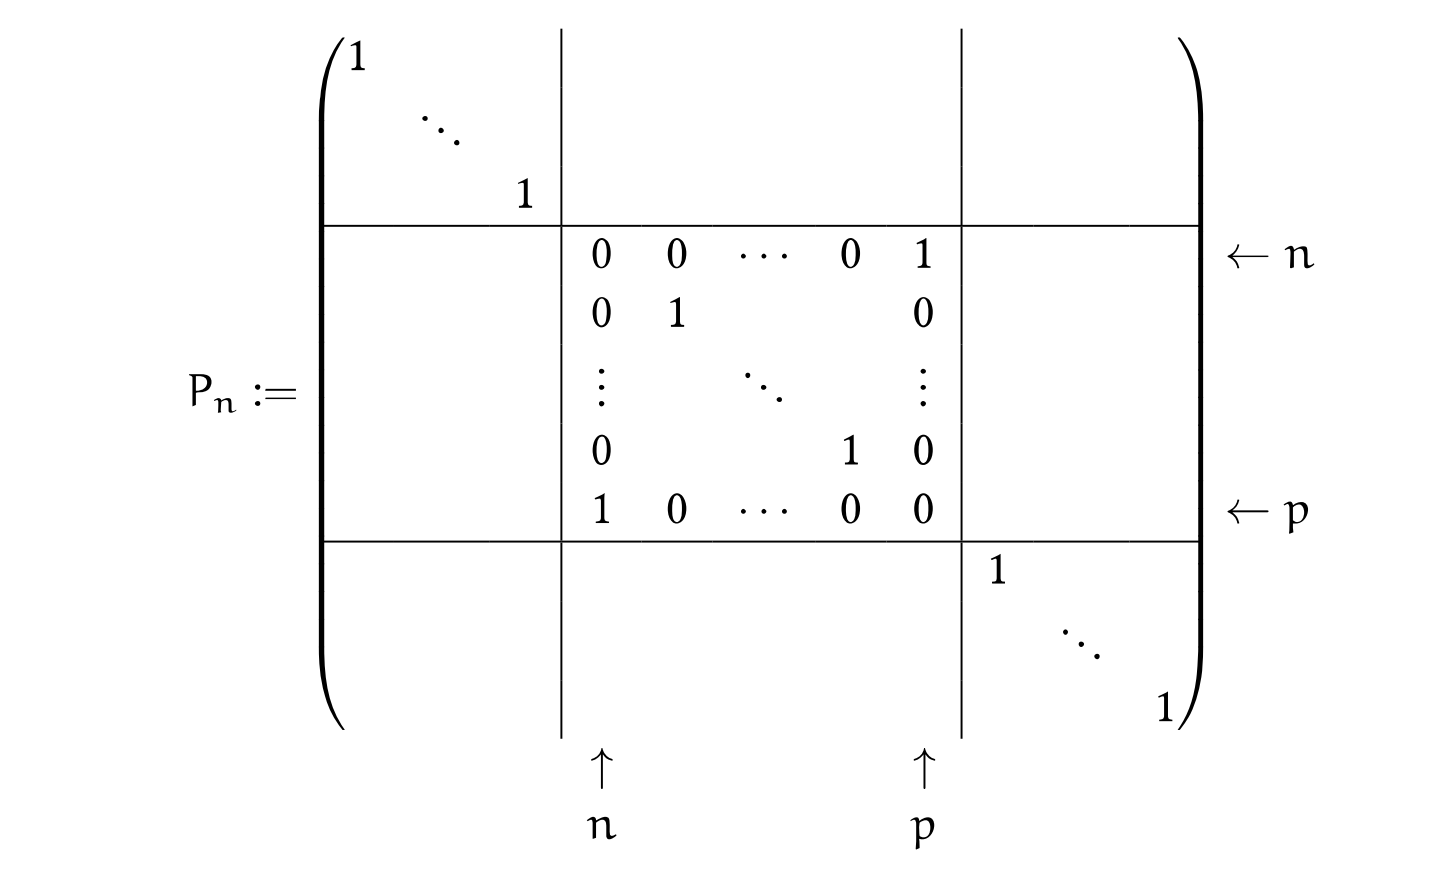
\includegraphics[scale=0.3]{permutation.png}
  \end{center}
  Die Matrix heißt elementare Permutationsmatrix und 
  hat folgende Eigenschaften: 
  \begin{itemize}
    \item $A\cdot P_n$ vertauscht n-te und p-te Zeile von A
    \item $P_n\cdot A$ vertauscht n-te und p-te Spalte von A
    \item $P^2_n = E_n$
  \end{itemize}
  Der n-te Schritt mit Pivotsuche ist daher:
  \[
    A^{(n+1)} = L_nP_nA^{(n)}
  \]
  Dann gilt für R und L:
  \[
    R := \tilde{L}_{N-1}\tilde{L}_{N-2}\cdots \tilde{L}_1PA 
      \hspace{0.5cm}\text{und} \hspace{0.5cm}
      L := \tilde{L}_{1}^{-1}\tilde{L}_{2}^{-1}\cdots
      \tilde{L}_{N-1}^{-1}
  \]
  mit 
  \[
    \tilde{L}_n := P_{N-1}\cdots P_{n+1}L_n P_{n+1} \cdots P_{N-1}
  \]
  Also gilt wieder: 
  \[
    PA = LR 
      \hspace{0.5cm}\text{dann läst man wieder} \hspace{0.5cm}
      Ly = Pb 
      \hspace{0.5cm}\text{und} \hspace{0.5cm}
      Rx = y
  \]
  Spaltenpivotsuche:\\
  Das m-te Pivotelement mit dem höchsten Score wird gewählt mit 
  der Sapltenmaximierungstrategie:
  \[
    \texttt{Pivoelement-Zeile} = 
    \texttt{argmax}_{n=m,\dots,N} = 
    \frac{|a_{n,m}|}{\sum_{l=m}^{N} = |a_{n,l}|}
  \]
}

\simplebox{LR-Zerlegung Algorithmus}{
  Algorithmus:
  \begin{enumerate}
    \item Start: $A^{(1)} := A$, $L^{(1)} := 0$, $P^{(1)} := E_N$
    \item Pivotsuche ergibt neues Element: 
        Vertausche Zeilen von $A^{(n)}$, also berechne: \\
          $A'^{(n)} := P_{n,j}A^{(n)}$,
          $P^{(n)} :=  P_{n,j}P^{(n-1)}$
    \item Pivotsuche gibt kein neues Element:
          $P^{(n)} := P^{(n-1)}$
    \item Berechne: 
      $l_n := \begin{pmatrix}
      0 \\ \vdots \\
      0 \\ \frac{a^{(n)}_{n+1,n}}{a^{(n)}_{n,n}} \\ \vdots\\
      \frac{a^{(n)}_{N,n}}{a^{(n)}_{n,n}} 
    \end{pmatrix}$,
      $L_n := 
      \begin{pmatrix}
        0  &   &  & &   \\
        &  \ddots &  &\\
        &  &  0 &  & & \\
        &  &  l_{n+1} & 0 & & \\
        &  &  \vdots & & \ddots & \\
        &  &  l_{N} & &  & 0&
      \end{pmatrix}$,
      $L_-^{(n)} := E_N - L^{(n)}$
    \item Berechne:  $A^{(n+1)} := L_-^{(n)}A^{(n)}$
    \item Schluss: $R := A^{(N)}$,
      $L = E_N + L^{(1)} + \cdots + L^{(N)}$
      , $P := P^{(N)}$
  \end{enumerate}
}

\simplebox{Cholesky Zerlegung}{
  Sei $A \in \mathbb{K}^{N\times N}$ hermitesch und
  positiv definit, dann gibt es eine untere Dreiecksmatrix 
  mit positiven Diagonalelementen und
  \[
    A = LL^*.
  \]
  Ansatz zur Berechnung:
  \[
    \begin{pmatrix}
      a_{1,1}& a_{1,2} &\cdots & a_{1,N} \\
      a_{2,1}& a_{2,2} &\cdots & a_{2,N} \\
      \vdots & \vdots &        & \vdots \\
      a_{N,1}& a_{N,2} &\cdots & a_{N,N} 
    \end{pmatrix}
    =
    \begin{pmatrix}
      l_{1,1}&  & & \\
      l_{2,1}& l_{2,2} &&\\
      \vdots & \vdots &  \ddots      & \\
      l_{N,1}& l_{N,2} &\cdots & l_{N,N} 
    \end{pmatrix}
    \cdot
    \begin{pmatrix}
      l_{1,1}&  \overline{l_{1,2}}& 
      \cdots& \overline{l_{1,N}}\\
            & l_{2,2} & \cdots&\overline{l_{2,N}}\\
      &    &  \ddots      & \vdots\\
      & &  & l_{N,N}
    \end{pmatrix}
  \]
  Mit Rechenaufwand:
  \[
    \texttt{Rechenaufwand} = \frac{1}{6}N^3 + \mathcal{O}(N^2)
  \]
}
\simplebox{Householder-Transformation} {
  Die Householder-Transformation bzgl. eines Vektors 
  $v \in \mathbb{K}^N$ ist: 
  \[
    P = E_n - \frac{2}{v^*v}vv^* \in \mathbb{K}^{N \times N}
  \]
  Die Householder-Transformation ist eine Spiegelung an 
  der Ebene orthogonal zu $v$.\\
  Für P gilt folgende Eigenschaften:
  \begin{itemize}
    \item $Pv = -v$
    \item $Pw=w$ $\forall w\perp v$
    \item P hermitesch, also $P^* = P$
    \item P unitär, also $P^*P = E_N$
  \end{itemize}
}

\simplebox{QR-Zerlegung}{
  Sei $A \in \mathbb{K}^{M \times N}$ mit 
  $M \geq N$ und $\texttt{rang}(A) = N$. Dann gibt es 
  eine unitäre Matrix $Q \in \mathbb{K}^{M\times M}$
  und eine obere Dreiecksmatrix $R \in \mathbb{K}^{M\times N}$
  mit 
  \[
    A = QR
  \]
  Wegen $Q$ unitär kann das Gleichungssystem wie folgt gelöst werden: 
  \[
    Rx = Q^*b
  \]
  Algorithmus:\\
  Im n-ten Schritt haben wir $A^{(n)}$ bestimmt und sei 
  $a_n = A_n^{(n)}$ die n-te Spalte von $A^{(n)}$.
  \begin{enumerate}
    \item Berechne $v_n := \frac{a_n}{||a_n||_2} + \delta_ne_1$ 
      mit $\delta_n := 
      \begin{cases}
        \frac{(a_n)_1}{|(a_n)_1|} &, (a_n)_1 \neq 0\\
        1 &, \text{sonst}
      \end{cases}
      $
    \item Berechne $\beta_n := \frac{2}{v^*v}$, $w_n := A^*v_n$
    \item Berechne $P_n = E_N - \beta_n v_nv_n^* = 
      \begin{pmatrix}
        E_n & 0 \\
        0  & P'_n
      \end{pmatrix}
      \implies 
      P_nA^{(n)} = A^{(n)} - \beta_n v_nw_n^* =
      \begin{pmatrix}
        r_{n,n} & * \\
        0  & A^{(n+1)}
      \end{pmatrix}
      $
    \item  Schluss: $R := P_n\cdots P_1A$ und 
      $Q := P_1\cdots P_n$
  \end{enumerate}
  Bemerkungen:
  \begin{itemize}
    \item QR-Zerlegung nicht eindeutig für $M \neq N$.
    \item Die Konditionszahl von der QR Zerlegung 
      ist gleich der von $A$, also 
      $\texttt{cond}_2(A) = \texttt{cond}_2(RQ)= \texttt{cond}_2(R)$.
    \item Also besser als bei der LR Zerlegung mit
      $\texttt{cond}_2(A) \leq \texttt{cond}_2(L) \texttt{cond}_2(R)$,
      wobei die Konditionszahlen von L und R viel höher als 
      A sein können.
    \item Auch besser als die Cholesky Zerlegung, da für die 
      cholesky-Zerlegung gilt: 
      $\texttt{cond}_2(A) \leq (\texttt{cond}_2(L'))^2 $.
    \item QR-Zerlegung ist doppelt so aufwendig wie LR-Zerlegung
      und viermal so aufwendig wie cholesky-Zerlegung.
    \item Falls der Rang nicht voll ist kann wieder 
      Vertauschungen von Spalten verwendet werden, um 
      den Algorithmus trotzdem anwendenden zu können.
    \item Der Algorithmus kann leicht abgewandelt werden 
      dass die Pivoelemente immer ungleich Null sind.
  \end{itemize}
  \[
    \texttt{Rechenaufwand} = MN^2 - \frac{1}{3} + \mathcal{O}(MN)
  \]
}

\simplebox{Lineare Ausgleichsrechnung} {
  Sei $Ax = b$ mit $A\in \mathbb{K}^{M \times N}$, 
  $x \in\mathbb{K}^N$, $b \in\mathbb{K}^M$ und 
  $M > N$. 
  Dieses LGS ist allgemein nicht lösbar, 
  deswegen brauchen wir einen neuen Lösungsbegriff:
  \[
    \inf_{x \in\mathbb{K}^N} ||Ax - b||_2
  \]
  Die Minimierer sind die Lösungen der Gaußschen 
  Normalengleichung:
  \[
    A^*Ax = A^*b
  \]
  Also eine Alternative zu der QR-Zerlegung
}
\simplebox{Banachscher Fixpunktsatz} {
  Sei $M$ vollständig bzg. einer Metrik $d$
  und sei $\phi: M \to M$ eine Abbildung, 
  sodass es ein $q > 1$ gibt mit
  \[
    \forall x,y \in M: d(\phi(x), \phi(y))
    \leq q \cdot d(x, y) 
\]
  Dann gibt es {\bf genau ein} $\hat{x} \in M$ mit 
  $\phi(\hat{x}) = \hat{x}$. Außerdem konvergiert für 
  jedes $x^{(0)} \in M$ die Folge
  \[
    x^{(n+1)} := \phi(x^{(n)}), \forall n\in \mathbb{N}_0
  \]
  gegen $\hat{x}$ und für $n \ge 1$ gilt:

  \begin{enumerate}[label=(\alph*)]
    \item Monotonie: $d(x^{(n)}, \hat{x}) 
      \leq q \cdot d(x^{(n-1)}, \hat{x})$
    \item A-priori-Schranke: $d(x^{(n)}, \hat{x})
      \leq \frac{q^n}{1-q} \cdot d(x^{(0)}, x^{(1)})$
    \item A-posteriori-Schranke: $d(x^{(n)}, \hat{x})
      \leq \frac{q}{1-q} \cdot d(x^{(n)}, x^{(n-1)})$
  \end{enumerate}
}
\simplebox{Fixpunktsatz angewendet auf lineare Gleichungssysteme}{
  Anwendung auf LGS $Ax = b$, zerlege in $A = M - N$.
  Daraus erhalten wir
  \[
    Mx = Nx +b.
  \]
  dass kann nun als ein Fixpunktproblem geschrieben werden: 
  \[
    x = Tx + c 
    \hspace{0.6cm} \text{mit}\hspace{0.3cm}  T = M^{-1}N 
    \hspace{0.3cm} \text{und}\hspace{0.3cm} c = M^{-1}x
  \]
  also $\phi(x) = Tx + c$.\\
  Dieses Problem konvergiert falls $||T||< 1$, für eine 
  induzierte Matrixnorm.\\\\
  Gesamtschrittverfahren(Jacobi-Verfahren): \\
  Hier ist $M = D$, $N = L+R$, wobei $D$ Diagonalmatrix 
  mit Einträgen ungleich Null, dann ist das wieder ein 
  Fixpunktproblem mit:
  \[ x_{\text{neu}} = D^{-1}(b + (L+R)x_{\text{alt}}\]
  \[ \iff x_{\text{neu}} = \underbrace{D^{-1}b}_{:= c}
  + \underbrace{D^{-1}(L+R)}_{:=T}x_{\text{alt}}\] 
  oder konkret:
  \[
    x_n^{(k+1)} = \frac{1}{a_{n,n}}
    (b_n - \sum_{\substack{m= 1 \\ m\neq n}}^{N} 
    a_{n,n}\cdot x_m^{(k)}) 
  \]
  Einzelschrittverfahren(Gauß-Seidel-Verfahren):\\
  Hier ist $M = D-L$ und $N = R$, daraus:
  \[
    x = (D-L)^{-1}(b-Rx)
  \]
  \[
    \rightsquigarrow x^{(neu)} = (D-L)^{-1}(b-Rx^{(alt)})
  \]
  \[
    \iff x^{(neu)} = D^{-1}(b+ Lx^{(neu)} - Rx^{alt})
  \]
  konkret:
  \[
    x_n^{k+1} = \frac{1}{a_{n,n}}(b_n - 
    \sum_{k=1}^{n-1}a_{n,m}x_m^{k+1} - 
    \sum_{k=n+1}^{N} a_{n,m} x_m^{k})
  \]
  Falls $A$ strikt diagonaldominant konvergieren 
  beide Verfahren für jeden Startwert $x^{(0)}\in \mathbb{K}^N$
}

\simplebox{Konjugierte Gradienten}{
  Sei $A \in \mathbb{K}^{N \times N}$ hermitesch und 
  positiv definit. Das Verfahren berechnet die exakte 
  Lösung wird aber oft vorher abgebrochen. \\
  Algorithmus: 
  \begin{enumerate}
    \item Start: Wähle $x^{(0)} \in \mathbb{K}^N$ 
      und setze $d^{(0)} := r^{(0)} = b - Ax^{(0)}$. 
      Ist $d^{(0)} = 0$ kann abgebrochen werden.
    \item Berechne: 
      \[
        \alpha_{k-1} := \frac{d^{(k-1)*} r^{(k-1)}}
        {d^{(k-1)*} A d^{(k-1)}}, \hspace{0.5cm}
        \beta_{k-1} := \frac{d^{(k-1)*} A r^{(k)}}
      {d^{(k-1)*} A d^{(k-1)}}
      \hspace{0.5cm}\text{und}\hspace{0.5cm}
      r^{(k)} := b - Ax^{(k)}
    \]
  \item Berechne: 
    \[
      x^{(k)} := x^{(k-1)} + \alpha_{k-1}d^{(k-1)}
      \hspace{0.5cm}\text{und}\hspace{0.5cm}
      d^{(k)} := r^{(k)} + \beta_{k-1}d^{(k-1)}
    \]
  \item Schluss: $d^{(k)} = 0 \implies x^{(k)} = \hat{x}$ 
    mit $A\hat{x} = b$
  \end{enumerate}
  Das Verfahren konvergiert nach genau $N$ schritten.\\
  Konvergenzrate:
  \[
    ||x^{(k)} - \hat{x}||_2 \leq 2 \texttt{cond}(A)
    \left(
    \frac{\sqrt{\texttt{cond}(A)} -1}{\sqrt{\texttt{cond}(A)}+1}
  \right)^k ||x^{0} -\hat{x}||_2
  \]

}

\simplebox{Eigenwerteinschließung} {
  Sei $A, \Delta A  \in \mathbb{K}^{N\times N}$, 
  $||\cdot||$ eine induzierte Matrixnorm und
  $\sigma(A) := \{\lambda \in \mathbb{C} : 
  \lambda \text{ ist Eigenwert von A} \}$.
  Dann gilt (Bauer-Fike):
  \[
    \min_{\lambda(A) \in \sigma(A)}|\lambda(A) - \mu(\Delta A)|
    \leq \texttt{cond}(A) \cdot ||\Delta A||.
  \]
  Wenn A \textit{normal} ($A^*A = AA^*$)  ist, so gilt sogar
  \[
    \min_{\lambda(A) \in \sigma(A)}|\lambda(A) - \mu(\Delta A)|
    \leq  ||\Delta A||_2.
  \]
  Gerschgorin:\\
  Sei
  \[
    \mathcal{K}_n := \{\xi \in \mathbb{C}: 
      |a_{n,n} - \xi|
      \leq 
      \sum_{\substack{m=1 \\ m\neq n}}^{N} |a_{n,m}|
    \}
    \hspace{0.5cm} \text{und} \hspace{0.5cm}
    \mathcal{K}^{*}_n := \{\xi \in \mathbb{C}: 
      |a_{n,n} - \xi|
      \leq 
      \sum_{\substack{m=1 \\ m\neq n}}^{N} |a_{m,n}|
    \}.
  \]
  Dann ist 
  \[
    \sigma(A) \subset \left(\bigcup_{n=1}^N \mathcal{K}_n
      \right) \cap  \left(\bigcup_{n=1}^N \mathcal{K}_n^*
      \right).
  \]
  Wenn $\mathcal{N}_1 \dot\cup \mathcal{N}_2 =  \{1,2, \dots,N\}$
  mit 
  \[
    \left(\bigcup_{n\in \mathcal{N}_1} \mathcal{K}_n
      \right) \cap  \left(\bigcup_{n \in \mathcal{N}_2}^N 
        \mathcal{K}_n^*
      \right) = \emptyset.
  \]
  Dann enthalten $\bigcup_{n \in \mathcal{N}_i}$, $i= 1,2$
  je genau $\#\mathcal{N}_i$ Eigenwerte.\\
  Courant-Fischer:\\
  Falls $A$ hermitesch mit Eigenwerten $\lambda_1 \geq 
  \lambda_2 \geq \dots \geq \lambda_N$. Dann gilt 
  für jeden Unterraum $\mathcal{L} \subset \mathbb{K}^N$
  mit $\texttt{dim}(\mathcal{L}) = n$, dass
  \[
    \min_{0\neq x \in \mathcal{L}} \frac{x^*Ax}{x^*x} \leq \lambda_n
    \hspace{0.5cm} \text{und} \hspace{0.5cm}
    \max_{0\neq x \in \mathcal{L}} \frac{x^*Ax}{x^*x} \geq \lambda_{N-n+1}
  \]
  mit Gleichheit $\mathcal{L}= \{x_1, \dots, x_n\}$ bzw. 
  $\mathcal{L}= \{x_{N-n+1}, \dots, x_N\}$, wobei 
  $(x_m)_{m=1}^{N}$ Eigenvektoren einer Orthonormalbasis sind.
}
\simplebox{Courant-Fischer Folgerung} {
  Sei $A, \Delta A  \in \mathbb{K}^{N\times N}$ 
  hermitesch, dann
  \[
    \lambda_n(A) + \lambda_N(\Delta A) 
    \leq \lambda_n(A + \Delta A) \leq 
    \lambda_n(A) + \lambda_1(\Delta A), \forall 
    n=1,\dots,N
  \]
  und insbesondere
  \[
    |\lambda_n(A+\Delta A) - \lambda_n(A)| 
    \leq ||\Delta A||_2 \forall 
    n=1,\dots,N
  \]
}
\simplebox{Potenzmethode} {
  \textit{Motivation}:
  Sei $A \in \mathbb{K}^{N \times N}$ diagonalisierbar,
  und $(v_n)_{n=1}^{N}$ eine Orthonormalbasis aus 
  Eigenvektoren, so gilt für $x = \sum_{n=1}^{N} \xi_n v_n$, dass 
  \[
    A^kx = \sum_{n=1}^{N} \lambda_n^k \xi v_n.
  \]
  Also dominiert der betragsgrößte Eigenwert für große 
  k.\\
  Sei $|\lambda_1| > |\lambda_2| \geq \dots \geq |\lambda_n|$
  die Eigenwerte von A, $0 \neq y \in \mathbb{C}^N$,
  mit $A^*y = \overline{\lambda_1}y$ und sei 
  $\tilde{z}^{(0)} \in \mathbb{C}^N$ mit 
  $y^*\tilde{z}^{(0)} \neq 0$,
  dann:
  \[
    z^{(k)} := \frac{A^k\tilde{z}^{(0)}}{||A^k\tilde{z}^{(0)}||},
    \forall k \geq 0
  \]
  so gilt 
  \[
    {\lim\sup}_{k \to \infty} |||Az^{(k)}|| - |\lambda_1|| \leq 
    \left(\frac{|\lambda_2|}{|\lambda_1|}\right)^k.
  \]
  Außerdem gibt es genau ein Eigenvektor von $\lambda_1$ mit 
  $||v|| = 1$ und $\texttt{sgn}(y^*v) = \texttt{sgn}(y^*\tilde{z}^{(0)})$
  und dann gilt:
  \[
    {\lim\sup}_{k \to \infty} ||z^{(k)} - \texttt{sgn}(\lambda_1)^kv|| \leq 
    \left(\frac{|\lambda_2|}{|\lambda_1|}\right)^k.
  \]
  Algorithmus:
  \begin{enumerate}
    \item Start: Wähle $\tilde{z}^{(0)}$, sodass möglichst 
      $y^*\tilde{z}^{(0)} \neq 0$
    \item Berechne $z^{k} := 
      \frac{\tilde{z}^{(k)}}{||\tilde{z}^{(k)}||}$
    \item Berechne $\tilde{z}^{(k)} := Az^{(k-1)}$
    \item Schluss Eigenwert: 
      $|\lambda_1| \approx ||Az^{(k)}||$
    \item Schluss Eigenvektor:
      $\texttt{sgn}(\lambda_1)^kz^{(k)} \approx v$
  \end{enumerate}
}
\dfn{Lokale Konvergenz} {
  Ein Iterationsverfahren $x_{k+1} = \phi(x_k)$, mit 
  $\phi(\hat{x}) = \hat{x}$
  heißt \textit{lokal Konvergent}
    gegen $\hat{x}\in \mathbb{K}$, falls es eine offene 
    Menge $U \subset \mathcal{D}(\phi)$ mit $\hat{x}\in U$
    gibt, sodass für jedes $x^{(0)} \in U$ das Iterationsverfahren
    definiert ist und gegen $\hat{x}$ konvergiert.
}
\dfn{Konvergenz Ordnung} {
  Ein lokal gegen $\hat{x}$ konvergentes Iterationsverfahren
  heißt konvergent \textit{von der Ordnung} $p \geq 1$,
  falls es ein $\rho > 0$ und $C < \infty$ (mit $C < 1$ für $p=1$)
  gibt mit:
  \[
    ||x_{k+1} - \hat{x}|| \leq C ||x_k - \hat{x}||^p, 
    \hspace{0.2cm}
    \forall k \geq 0 \hspace{0.2cm} \text{ und }\hspace{0.2cm}
    ||x_0 - \hat{x}|| < \rho
  \]
}
\ex{}{
  Das Gesamtschrittverfahren(Banach), Einzelschrittverfahren(Banach)
  und CG-Verfahren konvergieren mit Ordnung 1.
}
\simplebox{Konvergenz von Iterationsverfahren}{
    Falls $\phi: \mathcal{D}(\phi) \subset \mathbb{K}^N
    \to \mathbb{K}^N$ stetig differenzierbar mit 
    $\hat{x}$ im inneren von $\mathcal{D}(\phi)$ 
    und es gibt eine Induzierte Matrixnorm mit 
    $||\phi'(x)|| < 1$ so ist die Fixpunktiteration
    lokal konvergent gegen $\hat{x}$ \\
}
\simplebox{Ordnung von Iterationsverfahren}{
  Die Funktion $\phi: \mathcal{D}(\phi) \subset \mathbb{K}
    \to \mathbb{K}$  sie p-mal stetig differenzierbar
    mit $p \geq 2$ und habe einen Fixpunkt $\hat{x}$ im inneren
    von $\mathcal{D}(\phi)$. Ist 
    \[
      \phi'(x)= \dots = \phi^{(p-1)} = 0
    \]
    so ist die Fixpunktiteration lokal konvergent gegen 
    $\hat{x}$ mit Konvergenzordnung mindestens $p$.
    Ist zusätzlich $\phi^{(p)}(\hat{x}) \neq 0$, ist 
    die Ordnung genau $p$.
}

\simplebox{Newton-Verfahren}{
  Die Funktion $f: \mathcal{D}(\phi) \subset \mathbb{R}
  \to \mathbb{R}$ ist differenzierbar und sei 
  $\hat{x} \in \mathbb{R}$ mit $f(\hat{x}) = 0$, dann heißt folgende 
  Vorschrift \textit{Newton-Verfahren}:
  \[
    x_{k+1} := x_{k} - \frac{f(x_k)}{f'(x_k)}, \forall k\geq 0
  \]
  Falls $f \in C^3[a,b]$ und $\hat{x} \in (a,b)$ mit 
  $f(\hat{x}) = 0, f'(\hat{x}) \neq0 $. Dann konvergiert 
  das Newton-Verfahren lokal quadratisch, also $p = 2$, gegen 
  $\hat{x}$.\\
  Sekantenverfahren:\\
  \[
    x_{k+1} = x_k - \frac{x_k - x_{k-1}}{f(x_k) - f(x_{k-1})}f(x_k)
  \]
  Sei $-\infty < a < b \leq \infty$ und $f: [a,b) \to \mathbb{R}$
  stetig mit $f(a) = 0$ und in $(a,b)$ stetig differenzierbar
  $f'(x) > 0$ für alle $x \in (a,b)$. Außerdem gelte 
  \[
    f(x) \geq f'(x)(x-a) \forall x \in (a,b).
  \]
  Dann konvergiert das Newton-Verfahren für alle $x_0 \in (a,b)$
  gegen $a$ und die iterierte ist streng monoton fallend.
}

\simplebox{Polynom-Interpolation}{
  Seien $x_0, \dots, x_N \in \mathbb{R}$ 
  paarweise verschieden. Dann heißen
  $w(x) := \prod_{n=0}^{N}(x-x_n)$ das 
  knotenpolynom. \\
  Falls die Knoten angeordnet sind durch 
  $x_0<\dots <x_N$ heißt,
  \[
    l_n(x_k) := \frac{w(x_k)}{(x_k-x_n)w'(x_k)} = 
    \prod_{\substack{m=0\\ m\neq n}}^{N}
    \frac{x_k - x_m}{x_n - x_m} = \delta_{n,k}
  \]
  das Lagrange-Grundpolynom.
  Dann gibt es für alle $y_0, \dots, y_N \in \mathbb{K}$, 
  genau ein Polynom $p$ von $\texttt{Grad} \leq N$ mit
    \[
      p(x_n) = y_n, \forall n = 0, \dots, N.
    \]
    Dieses Polynom ist gegeben durch
    \[
      p(x) = \sum_{n=0}^{N} y_n l_n(x)
    \]
    Sei nun $f \in C^{N+1}[a,b]$ und $p$ das 
    Interpolationspolynom vom $\text{Grad} \geq N$.
    Dann gibt es zu jedem $x \in [a,b]$ ein 
    $\xi \in \texttt{conv}(x, x_0, \dots, x_N)$
    (Konvexehülle) mit 
    \[
      f(x) - p(x) = \frac{f^{(N+1)}(\xi)}{(N+1)1!} w(x).
    \]
    Insbesondere ist
    \[
    |f(x) -p(x)| \leq \frac{\max_{\xi \in [a,b]}|f(\xi)|}{(N+1)!} |w(x)|.
    \]
    Es gilt:
    \[
      \min_{x_0, \dots, x_n \in [a,b]} \max_{x\in [a,b]}
      |(x-x_0)\dots(x-x_N)| = \frac{(b-a)^{N+1}}{2\cdot 4^N}.
    \]
    Die beste Wahl ist dann für die Knoten:
    \[
      x_n = \frac{1}{2}\left(
        (b-a)\cos \frac{(2n-1)\pi}{2(N+1)} + a +b 
      \right)
      , n= 0,\dots, N
    \]
}
\dfn{Splines}{
  Sei $[a,b]$ Intervall und Knoten
  $a=x_0 < x_1< \dots < x_n =b$. Sei 
  \[
    h_n := x_n - x_{n-1}, n = 1, \dots, N
  \]
  und 
  \[
    h := \max_n h_n
  \]
  Ein Spline von Grad $L$  ist eine Funktion 
  $s \in C^{L-1}[a,b]$, die auf jeden Intervall
  $[x_{n-1}, x_n]$ mit einen Polynom von Grad $\geq L$ 
  übereinstimmt. Die Menge aller Splines vom Grad 
  $L$ wird mit  $S_L$ oder $S_{L,\Delta}$ mit 
  $\Delta = \{ x_0, \dots, x_N\}$ bezeichnet.\\
  $S_L$ ist ein $(N+L)$-dimensionaler Vektoraum.
}

\simplebox{Lineare Splines}{
  Hutfunktionen:
  \[
    \Lambda_0(x) = \begin{cases}
      \frac{x-x_1}{x_0 - x_1} &\text{falls } x_0 \leq x \leq x_1,\\
      0                       &\text{falls } x_1 \leq x \leq x_N
    \end{cases}
  \]
  \[
    \Lambda_n(x) = \begin{cases}
      0  &\text{falls } x_0 \leq x \leq x_{n-1},\\
      \frac{x-x_{n-1}}{x_{n} - x_{n-1}}  
         &\text{falls } x_{n-1} \leq x \leq x_n\\
      \frac{x-x_{n+1}}{x_{n} - x_{n+1}}
         &\text{falls } x_n \leq x \leq x_{n+1},\\
      0   &\text{falls } x_{n+1} \leq x \leq x_N
    \end{cases}
  \]
  \[
    \Lambda_N(x) = \begin{cases}
      0 &\text{falls } x_0 \leq x \leq x_{N-1},\\
      \frac{x-x_{N-1}}{x_N - x_{N-1}}   
        &\text{falls } x_{N-1} \leq x \leq x_N
    \end{cases}
  \]
}

\simplebox{Trigonomentrische Interpolation} {
  Sei O.B.d.A: $L= 2\pi$, $0 \leq \theta_0 < \theta_1 \dots 
    < \theta_{N-1} \leq L
  $
  und $y_0, \dots, y_{N-1}$.
  Zur Vereinfachung äquidistante Knoten:
  \[
    \theta_n = \frac{2\pi n}{N}
  \]

  


}

\end{document}
